\section{Základní nelinearity a popis nelineárních systémů (popis statických a dynamických nelineárních systémů,
vliv parazitních nelinearit na průběh regulačního děje)}

\subsection{bez dynamiky}
Systém reaguje na odezvu okamžitě, nebo je jeho časová konstanta výrazně nižší něž zbylé čas. konstanty.
Dělí se na :

\begin{itemize}
    \item bez paměti
    \item s pamětí
\end{itemize}

\subsubsection*{nelinearita bez paměti}

Dá se vyjádřit jako funkce 
\begin{equation}
    y=f(u)
\end{equation}

Na základě aktuální hodnoty se určí výstup. Dá se jednoduše linearizovat rozvojem da Taylorovi řady, nebo do polynomu.
popsána funkcí, grafem, tabulkou.
\\
např. :  saturace, tření\dots
\\
\\
\subsubsection*{nelinearita z pamětí}
Výstup záleží i na předchozích stavech, nelze jednoduše popsat jako funkce, často se popisuje slovně nebo jako algoritmus.
\\
např.: vůle v převodech, relé s hysterezí

\subsection*{Základní nelinearity}

\subsubsection*{nasycení(saturace)}
\begin{itemize}
    \item nejběžnější nelinearita (obsahuje ji v podstatě každý reálný systém)
    \item dá se s ní pracovat jako s po částech lineární funkcí
    \item pokud zajistíme že se systém nedostane z <b,a> lze prát jako lin. f-ce 
    \item např.: nádrž co přeteče
    \item (je jedním z faktorů pro vznik wind up jevu)
    \item bez paměti
\end{itemize}
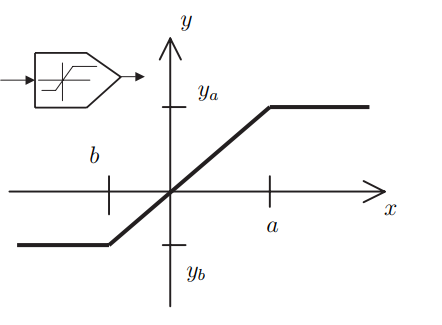
\includegraphics[]{img/saturace.png}

\subsubsection*{necitlivost}
\begin{itemize}
    \item nejčasttěji u mech systémů (projev tření a mech. nepřesností)
    \item např.: DC motor se roztočí až od určitého napětí
    \item občas se vkládá do reg. umělěle aby se omezili oscilace
    \item po částech lineární (většinou)
    \item bez paměti
\end{itemize}
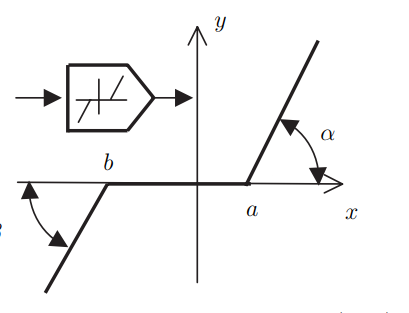
\includegraphics{img/necitlivost.png}

\subsubsection*{vůle v převodech (hystereze)}
\begin{itemize}
    \item při změně pohybu chvíli trvá než se něco začne dít
    \item v převodovkách, nebo při magnetizaci železa (hysterezní smyčka- v otázce MVE mag. měření)
    \item v převodovce lze odstranit tak že druhý motor tlačí vždycky proti
    \item rádi se na to ptají
    \item většinou nelze linearizovat
    \item s pamětí
\end{itemize}
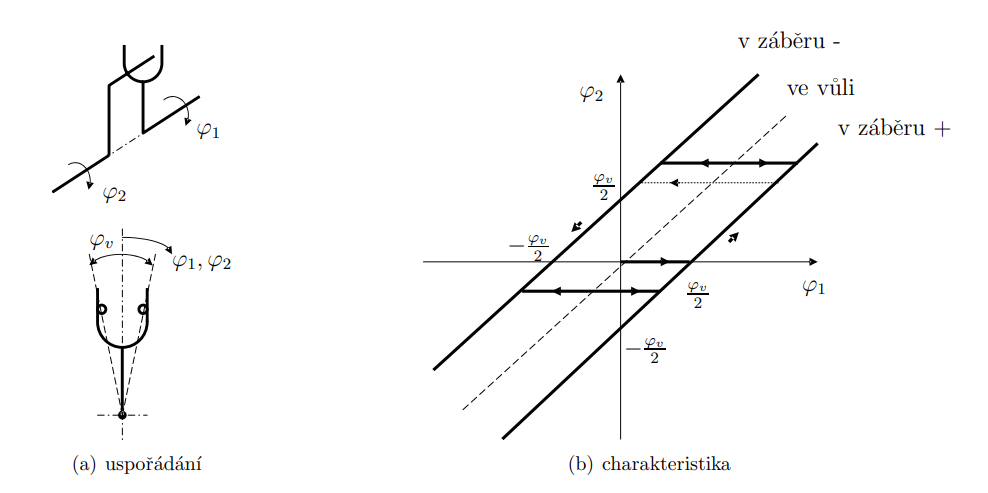
\includegraphics{img/vule.png}

\subsubsection*{tření}
\begin{itemize}
    \item v mech systémech
    \item špatně se linearizuje v okolí 0
    \item bez paměti
\end{itemize}
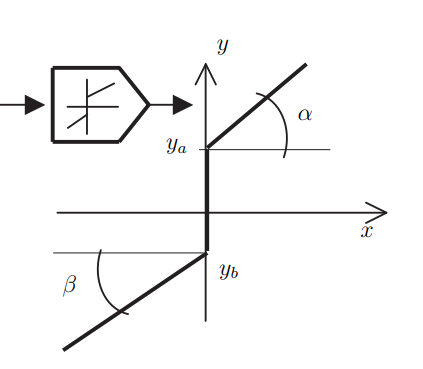
\includegraphics{img/treni.png}

\subsection*{releové charakteistiky}
\begin{itemize}
    \item s pamětí i bez
    \item požití jako regulátor
\end{itemize}
\includegraphics*{img/rele.png}

\subsection{s dynamikou}
popsány stavovými rovnicemi:
\[
    \frac{dx}{dt}=f(x,u)\]
    \[y=g(x,u)\]

\begin{itemize}   
    \item časově variantní
    \item časově invariantí (parametry se v čase nemění)
\end{itemize}
%----------------------------------
\newpage
\section{Ustálené chování nelineárních dynamických systémů (rovnovážné stavy, mezní cyklus, metoda
harmonické rovnováhy, stabilita mezního cyklu)}

Není v otázce přímo zmíněný ale asi dobrý vědět.

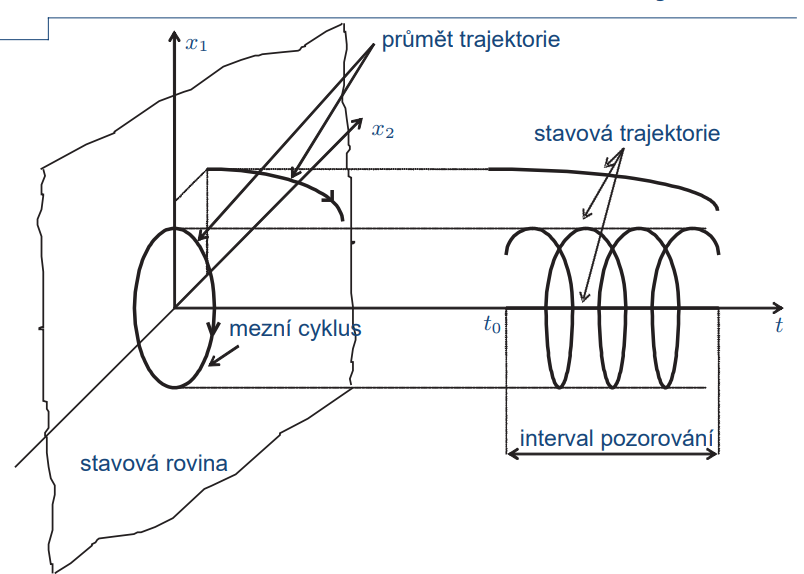
\includegraphics[scale = 0.8]{img/trajektorie.png}
{
\it stavová trajektorie (po systém 2. řádu) je 3d graf ukazuje jak se v čase mění vnitřní stavy systému.
Požívá se průmět stavové trajektorie, ukazuje jak se bude systém chovat, šipkou naznačeno odkud kam se bude v čase pohybovat.
}
\subsection{rovnovážný stav}
Stav systému, ktrý se v čase nemění. x=0 Průmět stavové trajektorie je bod. Určíme
ho jako \[ \dot{x} = 0 \]
Systém může mít o vice rovnovážných stavů, také nemusí mít žádný.

Rovnovážné stavy mohu být:
\begin{itemize}
    \item izolované - pokud kolem něj existuje jeho malé okolí ve kterém se nenachází další rovnovážný stav.
    \item neizolované
\end{itemize}

U rovnovážných stavů pak můžeme řešit jejich stabilitu, pokud se systém po drobném vychýlení do rovnaného 
stavu vrátí je rovnovážný stav stabilní.
O stabilitě/nestabilitě lze rozhodnout linearizací rozvojem do Taylorovi řady (podle polohy pólů náhrady)

\subsubsection{mezní cyklus}
Mezní cyklus nastává pokud se stavy systému periodicky opakují, průmět stav trajektorie je uzavřený obrazec (kruh).
Matematicky řečeno :
\[x(t+T)=x(t)\]
t-čas \\ T-perioda\\

Mezní cyklus muže být stabilní polostabilní nebo nestabilní:  

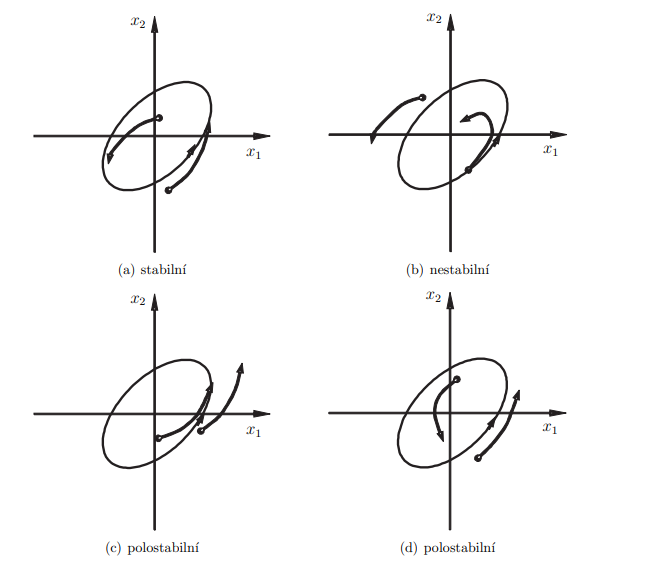
\includegraphics{img/mez_cykly.png}

Zda vzniknou mezní cykly jde určit metodou harmonické rovnováhy
\subsubsection*{metoda harmonické rovnováhy}
Vyžívá ekvivalentního přenosu nelinearity ke zkoumání mezních cyklů.

\subsubsection*{ekvivaletní přenos}
nelinearitu nahradíme ekvivalentním přenosem $N_e$, ten je závislá na Amplitudě vstupního signálu A.

Ekvivalentní přenos získáme  tak, že odezvu nelinearity na harmonický průběh o amplitudě A, převedeme pomocí Fourierovy transformace na jeho ekvivalentní přenos. U Fourierovy transformace uvažujeme pouze 1. harmonickou, 
protože se bere že další části obvodu mají charakter dolní propusti. Matematicky řečeno:
\begin{equation*}
    N_e= \frac{a_1+j\cdot b_1}{A}
\end{equation*}
kde
\begin{equation*}
    a_1=\frac{2}{T} \int_{0}^{T} f(e) \cdot sin(\omega t) dt
\end{equation*}

\begin{equation*}
    a_1=\frac{2}{T} \int_{0}^{T} f(e) \cdot cos(\omega t) dt
\end{equation*}

{\bf Tuto náhradu lze použít pouze pokud}
\begin{itemize}
    \item je dalším prvkem v regulačním obvodu systém typu dolní propust, který dostatečně potlačuje vyšší harmonické
    \item nelinearita při vstupním signálu $e=A\cdot sin (\omega t) $ negeneruje stejnosměrnou složku
\end{itemize}

Zjištění mezních cyklů 

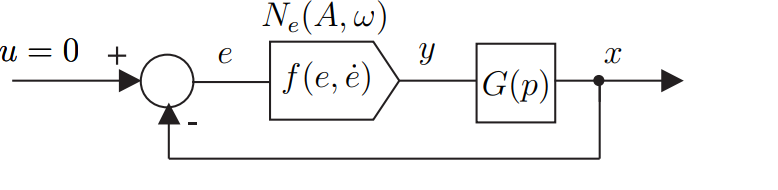
\includegraphics{img/harm.rovnovha.png}

Pro určení mezních cyklů musí být systém jako je na obrázku, kde f je nelinearita a G je lin přenos typu dolní propust.

Mezní cykly v systému vzniknou pokud bude "$ F_o =-1 $", tedy pokud bude výstup systému 
roven jeho výstupu posunutému o 180°, matematicky :
\begin{equation*}
    A= N_e \cdot G \cdot A
\end{equation*}
Úpravou dostaneme podmínku vzniku mezních cyklů jako :
\begin{equation*}
    G=\frac{-1}{N_e}
\end{equation*}
Tato rovnice často nelze numericky řešit a musí se řešit graficky.

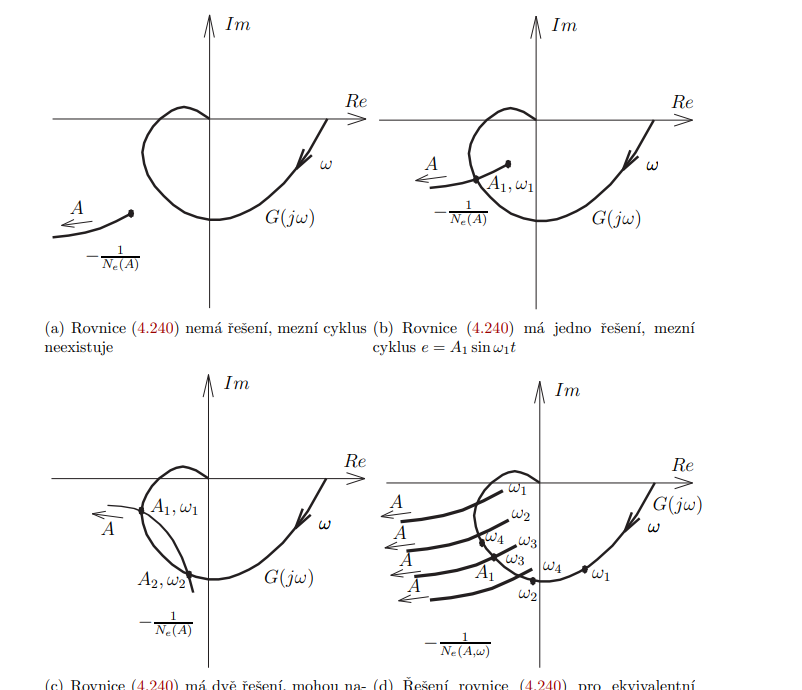
\includegraphics{img/garf.reseni.png}

dál lze touto metodou určit jestli je mezní cyklus stabilní, pomocí modifikovaného Nyquistova kritéria :
 například u bodu 1, pokud se sníží A dostaneme se do bodu 1'' pokud je charakteristika G nalevo do něj systém bude nestabilní tj amplituda se opět zvýší, pokud A zvýšíme dostane se do bodu 1' systém bude stabilní a amplituda se zmenší, mezní cyklus v bodě 1 je tedy stabilní.

 Tupě řečeno mezní cyklus je stabilní pokud se po snížení A nachází bod 1'' napravo od G a při zvýšení A se bod 1' nachází nalevo do G.
 mezní cyklus v bodě 1 je stabilní mezní cyklus v bodě 2 není.
 
 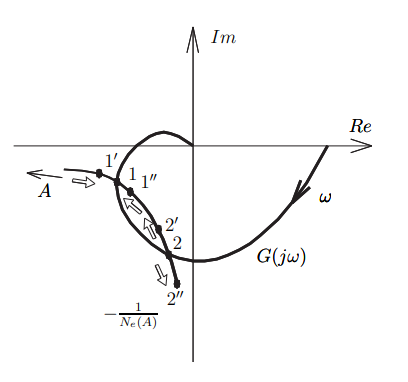
\includegraphics{img/stab.mez.cyklu.png}

 \section{Stabilita nelineárních systémů (definice, metody vyšetření, věty o nestabilitě, stabilita uzavřené regulační
 smyčky)}

 stabilitu určujeme podle Ljapunovových kritérií, ty platí pouze pro neřízené systémy.
 podle Ljapunova existují následující stability :

 \subsection{lokálně stabilní}
 Pokud v (libovolně malém) okolí $\varepsilon $ rovnovážného stavu $x_0$ vybereme počáteční bod $\delta $ jeho trajektorie dané okolí nepustí.

 \includegraphics{img/lok.stabilní.png}

 podle Václavka :

 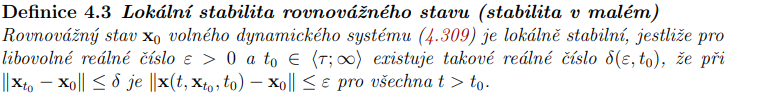
\includegraphics{img/vaclave.lok.png}

 \subsection{lokálně asymptoticky stabilní}
Systém je lokálně stabilní viz předchozí odstavec a zároveň platí že pro $t=\infty$ se systém dostane do $x_0$

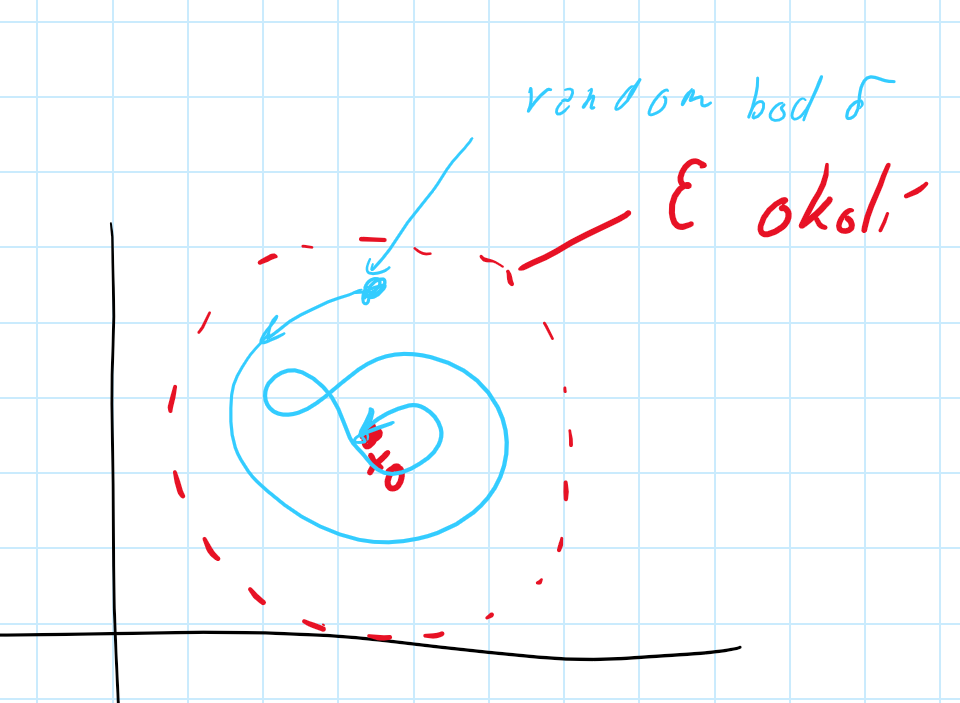
\includegraphics[scale = 0.6]{img/lok.asypt.stab.png}

podle Václavka:

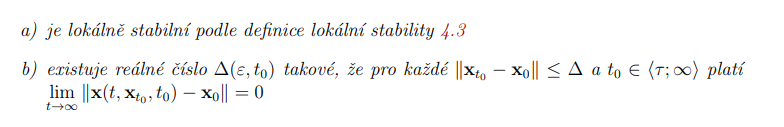
\includegraphics{img/vaclavek. lok.asypt..png}

\subsection{globálně  asymptoticky stabilní}
Pokud je systém lokálně asymptoticky stabilní a jeho okolí přitažlivosti (pokud v daném daného okolí umístíme systém skončí v $x_0$) zabírá 
celý stavový prostor.

jinými slovy pro libovolný bod stavového prostoru systém skončí v $x_0$.

podle Václavka

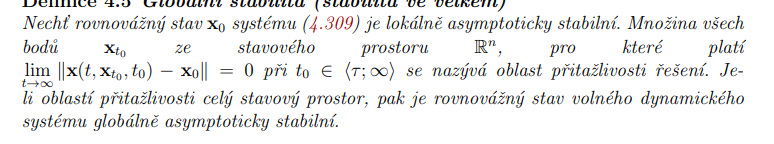
\includegraphics{img/vaclavek.golbal.png}

Tato podmínka je docela tvrdá, proto se zavádí Praktická stabilita, systém je prakticky stabilní v oblasti $\Omega$ pokud je lokálně asymptoticky stabilní a má oblast přitažlivosti $\Omega$.

\subsection*{určení stability}
Jedná pouze o podmínky postačující pro stabilitu, pokud tedy systém podmínce nevyhoví nelze o něm říct že je nestabilní.
\subsubsection{I Ljapunovovo kritériu stability}
Určuje stabilitu systému na základě stability linearizované náhrady v okolí rovnovážného stavu.

\noindent 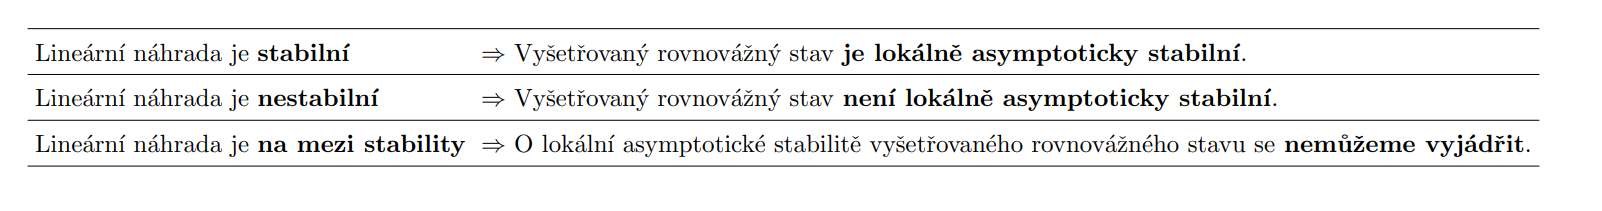
\includegraphics[scale = 0.6]{img/Ljap.1.png}

\subsubsection{II Ljapunovovo kritériu stability}
Určíme si fukci V aby byla pozitivně
 definitní (PD), spočítáme W jako gradient V (v podstatě spíš derivaci ale ve skriptech to mají nazváno gradiet). Podle toho jestli je w ND , NSD určíme stabilitu.

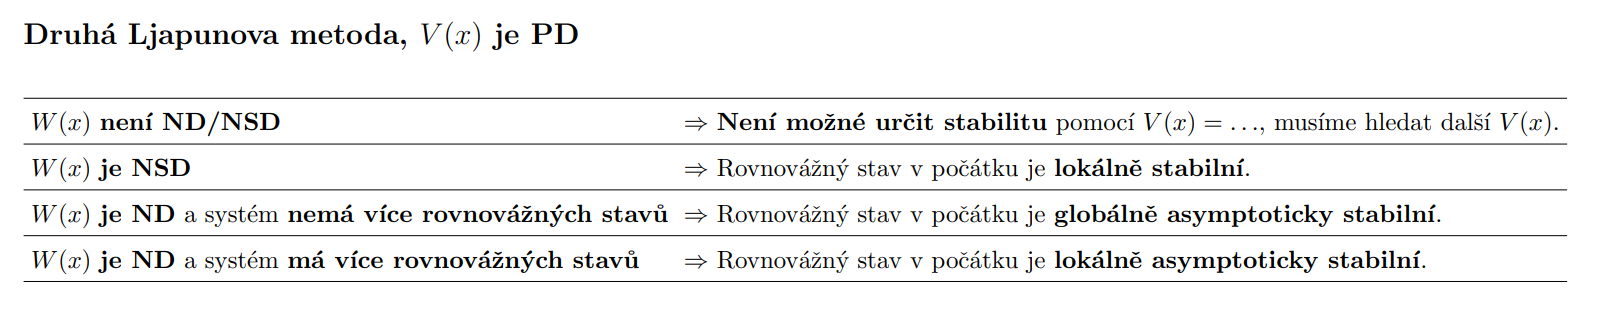
\includegraphics[scale = 0.6]{img/Ljap.2.png}

V můžeme volit náhodně nebo lze využít {\bf Krasovského metodou}, kde V zvolíme jako součin námi zvolené matice L a funkcí f, které získáme ze stavových rovnic.
L musí být symetrická a PD. Matamatickými čáry pak dostaneme že W bude ND pokud T bude PD.
T spočítáme jako :
\begin{equation*}
    T=J^TL+JL
\end{equation*}

další metodu volby V je {\bf metoda variabilního gradientu } to ale doufám že umět nemusíme.

\subsubsection{Popovo kritérium stability}
Aby byl podle popova systém stabilní musí být splněno:
\begin{itemize}
    \item systém je neřízený
    \item systém  je v konfiguraci jak je na obr.

        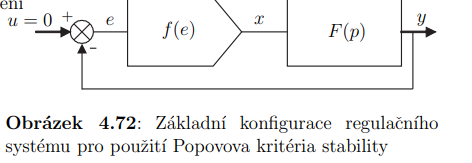
\includegraphics{img/popov.schem.png}
    \item hodnota nelinerity v 0 je 0 $f(0)=0$
    \item průbeh nellinearity je "pod" přímkou procházející počátkem se směrnicí k

        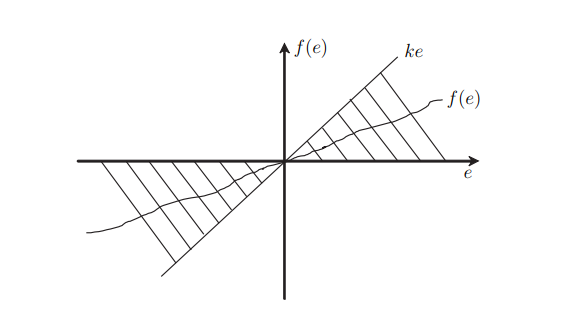
\includegraphics{img/popov_nelilin.png}
    \item modnifikovaná frekvenční charakteristika $f^*=Re{F}+j\omega Im{F}$ (F je frekvenční charakteristika zkoumaného systému) se musí nacházet pod popovovou přímkou,
    ta může mít libovolný sklon a musí procházet bodem -1/k

        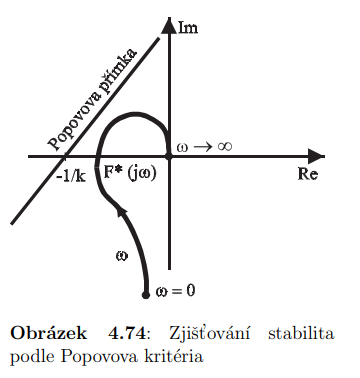
\includegraphics{img/popov_frek.png}
\end{itemize}
pod jsou všechny podmínky splněny systém je globálně asymptoticky stabilní.

\subsection{věty o nestabilitě}
Opět se jedná pouze o postačující podmínky, pokud jim systém nevyhoví nevíme nic.

\subsubsection{I Ljapunovova věta o o nestabilitě}
podud exzistuje funkce V pro kterou platí :
\begin{itemize}
    \item V(0)=0
    \item $\frac{dV}{dt}$ je PD
    \item V není ND nebo NSD v libovolně málem okolí počátku
\end{itemize}
poto je rovnovážný bod v počátku nestabilní.

\subsubsection{II Ljapunovova věta o o nestbilitě}
pokud V není ND , nebo NSD, a její derivace je PSD, je rovnovážný bod v počátku nestabilní.
* V musí být spojitá a musí mít spojitou 1. derivaci.
\subsubsection{četajevoa věta o nestabilitě}
vůbec nechápu

%------------------------
\section{Reléová regulace (on-off regulátory, řízení v klouzavém režimu).
}

Jako regulátor je použito relé, nebo jiný spínací prvek, chovající se stejně. 
Použije se pokud akční zásah nabývá jen 2 hodnot (on-off control),nebo pokud akční veličina max kladné nebo max záporné hodnoty (bang-bang control).

Nejtypičtější využití regulace teploty (žehlička, topení), tlak v kompresorech se zásobníkem.
Možné varianty relé jsou o dvě otázky víš.

Pokud bychom chtěli regulovat např teplotu pomocí klasického relé, neustále by spínalo  (i vlivem šumu), proto je lepší použít relé s hysterezi, podle šířky hystereze můžeme nastavit s jakou periodou bude kmitat.

Pokud nám u řízení pomocí relé s hysterezí nevyhovuje nastavení hystereze a z nějakýho (nepochopitelného) důvodu ji nemůžeme měnit lze chování upravit přidáním setrvačného článku do zpětné vazby.
Musí platit že oba přepínací body jsou větší než 0, potom při sepnutí relé dojde ke zpoždění informace ve zpětný vazbě a relé sepne zpět až později. Časová konstanta setrvačného článku musí být malá.

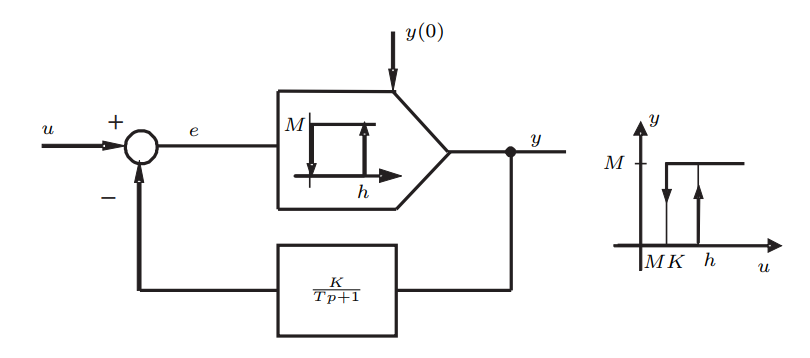
\includegraphics{img/rele_reg.png}

{ \it
Pokud řídím polohu a chci stihnou zastavit včas, může být přivedená další zpětná vazba od rychlosti, touhle hodnotou si upravím kdy bude relé spínat.
}

pro návrh reléového regulátoru lze využít např Lipanova...

Pro složitější systémy se využívá {\bf řízení v klouzavém režimu}
Relé je nastaveno tak, aby se systém dostal na přepínací rozhraní  po přepínacím rozhraní došel až do 0.

 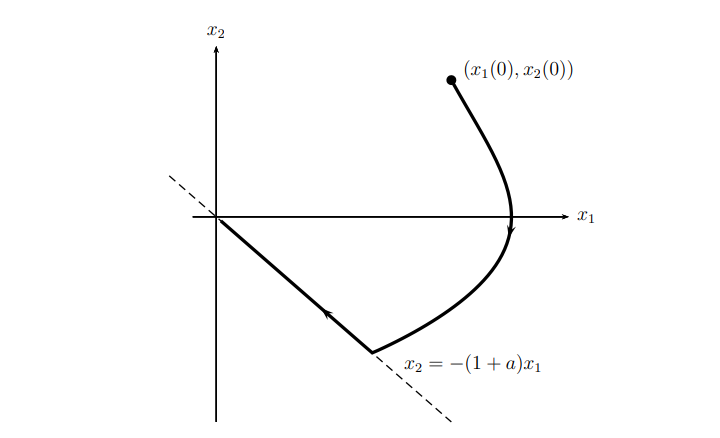
\includegraphics{img/kluzavy_obr.png}

 \begin{itemize}
    \item systém může obsahovat neurčitost -> jedná se o robustní řízení
    \item musím být schopen měřit aktuální hodnotu vnitřních stavů
    \item na přepínacím rozhraní kmitá relé nesmyslně rychle, proto se nahrazuje něčím pozvolnějším 

    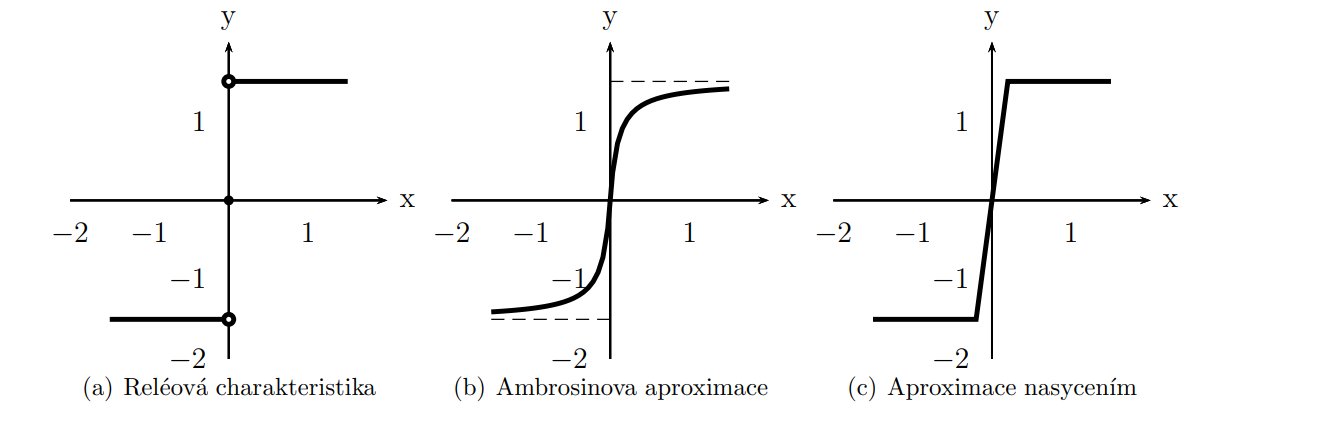
\includegraphics[scale = 0.5]{img/kluzavy_rele.png}

 \end{itemize}

obeně postup návrhu řízení v klouzavém režimu
\begin{enumerate}
    \item popis systému převedeme na požadovaný tvar (oddělené neurčitosti $\delta $ od zbylých závislostí)
    
    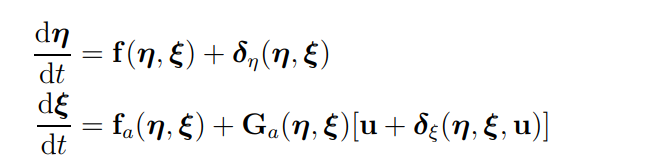
\includegraphics[scale =0.4]{img/klouzavy_tavr.png}
    \item navrhneme řízení systému na který může působit přímo vstupem - tím definujeme přepínací rozhraní
    \item zavedeme proměnou co určuje odchylku od přepínacího rozhraní, její derivací získáme "systém", který musí směřovat do 0 (navrhneme pro něj takové řízení)
    \item určíme ekvivalentní řízení $u_{eq}$, tak aby v rovnici došlo k eliminaci známých členů
    \item dosadíme získáme $\Delta$
    \item určíme max $\Delta$ 
    \item dosadíme, určíme řízení (předpis pro regulátor) V

\end{enumerate}

%-----------------------------------
\section{Linearizace nelineárních dynamických systémů (rozvoj do Taylorovi řady, exaktní zpětnovazební
linearizace).
}

\subsection{Linearizace do Taylorovi řady}
\begin{itemize}
    \item nejrozšířenější 
    \item linearizuje systém pouze v okolí daného bodu
    \item vstupní výstupní vektory linearizovaného systému odpovídají { \bf odchylkám} od bodu ve kterém linearizujeme
    \item pro linearizaci využijeme pouze prví člen Taylorovi rady, ostatní zanedbáváme.
    \item výpočet se provádí pomocí parciálních derivací jednotlivých rovnic- Jakobyho matice
\end{itemize}

\subsection{exaktní zpětnovazební linearizace}
oproti rozvoji do Taylorovi řady popisuje celý systém, ale musíme znát hodnoty vnitřních stavů.
\subsubsection{cstup-stav}
Spočívá v tom že zavedeme nový vstup u ,ten bude osahovat opravdový vstup v + další prvky, které nahradí nelinearity.
Diferenciální r-ce je potřeba upravit tak(substituce, transformace), aby nelineární část byla jen v rovnici kde je u, potom napíšeme vhodné u.
Př.:
zadaný systém:
\begin{equation}
    \dot{x_1}=cokoliv lineárního
\end{equation}
\begin{equation*}
    \dot{x_2}=x_1+2x_2+cos(x_2)+u
\end{equation*}
řešení
\begin{equation*}
    \dot{x_1}  zůstává
\end{equation*}
\begin{equation}
    \dot{x_2}=x_1+2x_2+u
\end{equation}
\begin{equation*}
    u=v+cos(x_2)
\end{equation*}

někdy můžou být úpravy hodně složité

\subsubsection{linearizace vstup-výstup}
zajímá nás pouze jak se chová výstup v závislosti na vstupu. Postupně derivujeme výstup dokud nedostaneme závislost na vstupu.

Může dojít k tomu že aproximovaný systém bude nižšího řádu něž byl původně, tj systém bude mít skrytou vnitřní dynamiku to může působit problémy.

\includegraphics[scale =0.6]{img/vstup-výstup1}

\includegraphics[scale =0.6]{img/vstup-výstup2.png}


